%%%%%%%%%%%%%%%%%%%%%%%%%%%%%%%%%%%%%
% Tracing Overhead
%%%%%%%%%%%%%%%%%%%%%%%%%%%%%%%%%%%%%

\subsection{Tracing Overhead}
\label{subsec:lowtoh}
\iffalse

\begin{table*}[]
\caption{Req BW}
\label{comet_bw_pMpAcg_BC_itn_p3.5}\begin{center}
\begin{tabular}{lrrrrrrrrr}
\hline
                &    bt &     cg &    ep &    ft &    is &     lu &    mg &     sp &    GM \\
\hline
 pinMain.B.1    &  4.72 &  21.86 &  3.83 &  1.52 &  0.79 &   2.39 &  5.62 &   5.36 &  3.69 \\
 pinMain.B.4    & 14.28 &  41.08 &  1.89 &  3.48 &  2.24 &  21.48 &  6.45 &  15.85 &  8.12 \\
 pinMain.B.16   & 14.31 &  46.59 &  1.45 &  4.86 &  3.40 &  31.79 &  6.53 &  18.55 &  9.41 \\
 pinMain.B.64   & 18.56 &  43.59 &  1.25 &  4.56 &  4.49 &  27.07 &  5.63 &  29.62 &  9.92 \\
 AVG            & 12.97 &  38.28 &  2.10 &  3.60 &  2.73 &  20.68 &  6.06 &  17.35 &  7.79 \\
 pinAll.B.1     & 48.71 &  89.39 & 47.23 & 45.63 & 59.98 &  53.62 & 60.81 &  54.33 & 56.21 \\
 pinAll.B.4     & 61.84 & 101.23 & 45.21 & 55.12 & 53.20 &  71.09 & 54.85 &  73.62 & 62.68 \\
 pinAll.B.16    & 73.95 & 116.87 & 47.37 & 48.88 & 47.79 & 100.91 & 55.80 &  84.61 & 67.97 \\
 pinAll.B.64    & 81.80 & 110.15 & 44.16 & 47.98 & 37.84 & 100.26 & 52.67 &  99.90 & 66.47 \\
 AVG            & 66.58 & 104.41 & 45.99 & 49.40 & 49.70 &  81.47 & 56.03 &  78.12 & 63.33 \\
 callgrind.B.1  &  1.57 &   7.69 &  7.39 &  4.56 & 39.49 &   2.61 & 34.41 &   2.71 &  6.67 \\
 callgrind.B.4  &  6.51 &  16.01 & 22.10 & 15.65 & 45.46 &   8.63 & 45.47 &   7.78 & 16.31 \\
 callgrind.B.16 & 17.20 &  24.62 & 37.42 & 23.84 & 29.87 &  16.23 & 51.49 &  15.81 & 24.93 \\
 callgrind.B.64 & 26.82 &  27.65 & 45.93 & 25.14 & 11.04 &  17.75 & 45.27 &  20.20 & 25.02 \\
 AVG            & 13.03 &  18.99 & 28.21 & 17.30 & 31.47 &  11.30 & 44.16 &  11.62 & 18.23 \\
 pinMain.C.1    &  1.82 &  16.96 &  5.15 &  1.16 &  0.69 &   0.77 &  3.56 &   1.40 &  2.17 \\
 pinMain.C.4    &  7.53 &  44.87 &  3.00 &  2.50 &  2.12 &  20.13 &  7.08 &  13.74 &  7.55 \\
 pinMain.C.16   & 16.30 &  55.04 &  1.84 &  6.10 &  3.35 &  34.09 &  7.24 &  20.68 & 10.70 \\
 pinMain.C.64   & 17.45 &  61.43 &  1.30 &  5.93 &  4.42 &  38.28 &  5.62 &  26.09 & 10.94 \\
 AVG            & 10.77 &  44.58 &  2.82 &  3.92 &  2.65 &  23.32 &  5.88 &  15.48 &  7.84 \\
 pinAll.C.1     & 17.80 &  53.37 & 26.34 & 20.89 & 48.31 &  25.31 & 52.61 &  19.46 & 29.99 \\
 pinAll.C.4     & 51.78 &  95.84 & 36.80 & 43.82 & 51.40 &  58.39 & 54.18 &  65.77 & 55.15 \\
 pinAll.C.16    & 75.38 & 121.03 & 44.29 & 61.39 & 46.90 & 101.05 & 56.49 & 101.32 & 71.37 \\
 pinAll.C.64    & 80.63 & 135.19 & 43.49 & 46.28 & 37.09 & 117.87 & 54.05 &  99.02 & 68.99 \\
 AVG            & 56.40 & 101.36 & 37.73 & 43.09 & 45.93 &  75.66 & 54.33 &  71.39 & 56.38 \\
 callgrind.C.1  &  0.40 &   3.09 &  1.96 &  1.05 & 14.60 &   0.70 &  6.96 &   0.75 &  1.85 \\
 callgrind.C.4  &  1.78 &   8.87 &  7.74 &  4.48 & 31.74 &   2.82 & 21.03 &   2.78 &  6.41 \\
 callgrind.C.16 &  6.01 &  15.82 & 22.86 & 10.75 & 26.50 &   7.45 & 39.05 &   6.96 & 13.72 \\
 callgrind.C.64 & 14.32 &  19.56 & 35.75 & 12.17 & 11.07 &  11.86 & 40.69 &  12.83 & 17.39 \\
 AVG            &  5.63 &  11.84 & 17.08 &  7.11 & 20.98 &   5.71 & 26.93 &   5.83 &  9.84 \\
\hline
\end{tabular}
\end{center}
\end{table*}

\fi


\iftrue

\begin{table*}[]
\caption{ Required Bandwidth per core (kB/s) }
\label{comet_bw_pMpAcg_BC_itn_p3.5}\begin{center}
\npdecimalsign{.}
\nprounddigits{1}

\begin{tabular}{|c|c|c|n{3}{1}n{3}{1}n{3}{1}n{3}{1}n{3}{1}n{3}{1}n{3}{1}n{3}{1}|n{3}{1}|}
\hline
Input & Tool & \# Nodes  & \multicolumn{1}{c}{bt} & \multicolumn{1}{c}{cg} & \multicolumn{1}{c}{ep} & \multicolumn{1}{c}{ft} & \multicolumn{1}{c}{is} & \multicolumn{1}{c}{lu} & \multicolumn{1}{c}{mg} & \multicolumn{1}{c|}{sp} & \multicolumn{1}{c|}{GM} \\ \hline
\multirow{15}{*}{B} & \multirow{5}{*}{ParLOT(m)} & 1 &  4.72 &  21.86 &  3.83 &  1.52 &  0.79 &   2.39 &  5.62 &   5.36 &  3.69 \\
 & & 4                                               & 14.28 &  41.08 &  1.89 &  3.48 &  2.24 &  21.48 &  6.45 &  15.85 &  8.12 \\
 & & 16                                              & 14.31 &  46.59 &  1.45 &  4.86 &  3.40 &  31.79 &  6.53 &  18.55 &  9.41 \\
 & & 64                                              & 18.56 &  43.59 &  1.25 &  4.56 &  4.49 &  27.07 &  5.63 &  29.62 &  9.92 \\ \cline{3-12} 
 & & AVG                                             & 12.97 &  38.28 &  2.10 &  3.60 &  2.73 &  20.68 &  6.06 &  17.35 &  {\boldmath}7.79  \\ \cline{2-12} 
 & \multirow{5}{*}{ParLOT(a)} & 1 & 48.71 &  89.39 & 47.23 & 45.63 & 59.98 &  53.62 & 60.81 &  54.33 & 56.21 \\
 & & 4                            & 61.84 & 101.23 & 45.21 & 55.12 & 53.20 &  71.09 & 54.85 &  73.62 & 62.68 \\
 & & 16                           & 73.95 & 116.87 & 47.37 & 48.88 & 47.79 & 100.91 & 55.80 &  84.61 & 67.97 \\
 & & 64                           & 81.80 & 110.15 & 44.16 & 47.98 & 37.84 & 100.26 & 52.67 &  99.90 & 66.47 \\ \cline{3-12} 
 & & AVG                          & 66.58 & 104.41 & 45.99 & 49.40 & 49.70 &  81.47 & 56.03 &  78.12 & {\boldmath}63.33 \\ \cline{2-12} 
 & \multirow{5}{*}{Callgrind}  & 1  &  1.57 &   7.69 &  7.39 &  4.56 & 39.49 &   2.61 & 34.41 &   2.71 &  6.67  \\
 & & 4                              &  6.51 &  16.01 & 22.10 & 15.65 & 45.46 &   8.63 & 45.47 &   7.78 & 16.31  \\
 & & 16                             & 17.20 &  24.62 & 37.42 & 23.84 & 29.87 &  16.23 & 51.49 &  15.81 & 24.93  \\
 & & 64                             & 26.82 &  27.65 & 45.93 & 25.14 & 11.04 &  17.75 & 45.27 &  20.20 & 25.02  \\ \cline{3-12} 
 & & AVG                            & 13.03 &  18.99 & 28.21 & 17.30 & 31.47 &  11.30 & 44.16 &  11.62 & {\boldmath}18.23  \\ \hline
 \multirow{15}{*}{C} & \multirow{5}{*}{ParLOT(m)} & 1  &  1.82 &  16.96 &  5.15 &  1.16 &  0.69 &   0.77 &  3.56 &   1.40 &  2.17  \\
 & & 4                                                 &  7.53 &  44.87 &  3.00 &  2.50 &  2.12 &  20.13 &  7.08 &  13.74 &  7.55  \\
 & & 16                                                & 16.30 &  55.04 &  1.84 &  6.10 &  3.35 &  34.09 &  7.24 &  20.68 & 10.70  \\
 & & 64                                                & 17.45 &  61.43 &  1.30 &  5.93 &  4.42 &  38.28 &  5.62 &  26.09 & 10.94  \\ \cline{3-12} 
 & & AVG                                               & 10.77 &  44.58 &  2.82 &  3.92 &  2.65 &  23.32 &  5.88 &  15.48 &  {\boldmath}7.84  \\ \cline{2-12} 
 & \multirow{5}{*}{ParLOT(a)} & 1 & 17.80 &  53.37 & 26.34 & 20.89 & 48.31 &  25.31 & 52.61 &  19.46 & 29.99 \\
 & & 4                            & 51.78 &  95.84 & 36.80 & 43.82 & 51.40 &  58.39 & 54.18 &  65.77 & 55.15 \\
 & & 16                           & 75.38 & 121.03 & 44.29 & 61.39 & 46.90 & 101.05 & 56.49 & 101.32 & 71.37 \\
 & & 64                           & 80.63 & 135.19 & 43.49 & 46.28 & 37.09 & 117.87 & 54.05 &  99.02 & 68.99 \\ \cline{3-12}
 & & AVG                          & 56.40 & 101.36 & 37.73 & 43.09 & 45.93 &  75.66 & 54.33 &  71.39 & {\boldmath}56.38  \\ \cline{2-12} 
 & \multirow{5}{*}{Callgrind} & 1 &  0.40 &   3.09 &  1.96 &  1.05 & 14.60 &   0.70 &  6.96 &   0.75 &  1.85  \\
 & & 4                            &  1.78 &   8.87 &  7.74 &  4.48 & 31.74 &   2.82 & 21.03 &   2.78 &  6.41  \\
 & & 16                           &  6.01 &  15.82 & 22.86 & 10.75 & 26.50 &   7.45 & 39.05 &   6.96 & 13.72  \\
 & & 64                           & 14.32 &  19.56 & 35.75 & 12.17 & 11.07 &  11.86 & 40.69 &  12.83 & 17.39  \\ \cline{3-12}
 & & AVG                          &  5.63 &  11.84 & 17.08 &  7.11 & 20.98 &   5.71 & 26.93 &   5.83 &  {\boldmath}9.84  \\ \hline
\end{tabular}
\end{center}
\end{table*}

\fi


%%%%%%%%%%%%%%%%%%%%%%%%%%%%%%%%%
% FROM RESULTS - average bandwidth
%%%%%%%%%%%%%%%%%%%%%%%%%%%%%%%%%
\begin{figure}[t]
\centering
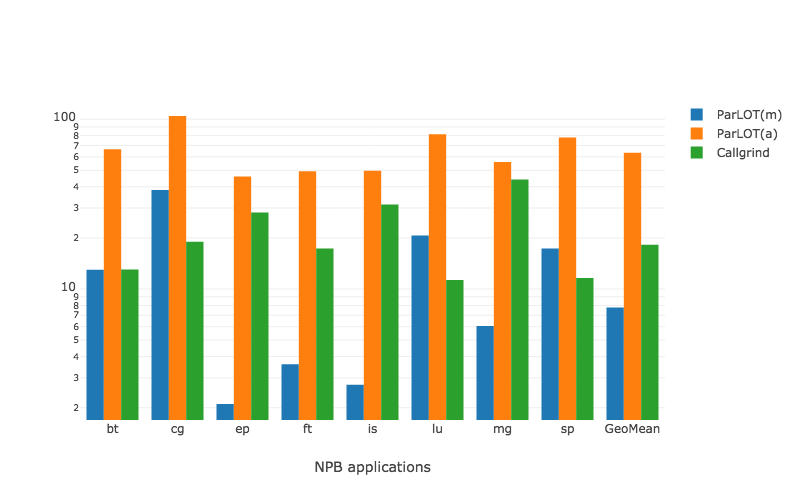
\includegraphics[width=3.8in]{figs.comet.newMed/comet_chartAvg_bw_B_p3_5.png}
\caption{  Average required bandwidth per core (kB/s) on the NPB applications - Input B}
\label{comet_chartAvg_bw_B_p3_5}
\end{figure}

\begin{figure}[t]
\centering
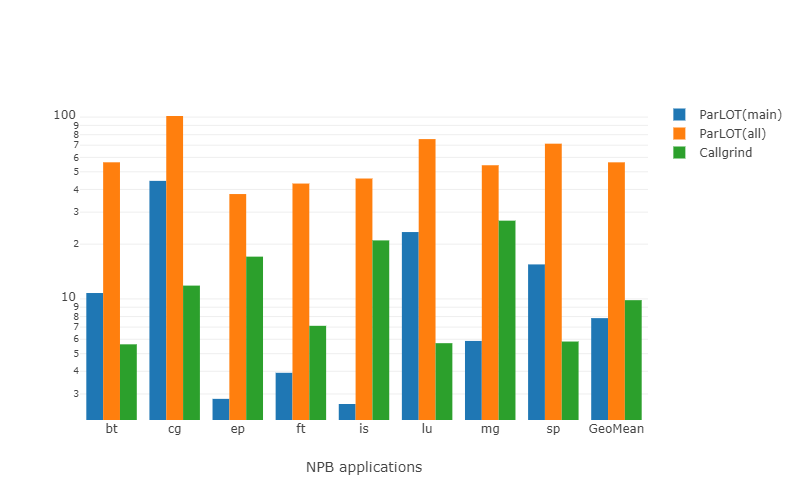
\includegraphics[width=3.8in]{figs.comet.newMed/comet_chartAvg_bw_C_p3_5.png}
\caption{ Average required bandwidth per core (kB/s) on the NPB applications - Input C}
\label{comet_chartAvg_bw_C_p3_5}
\end{figure}

%%%%%%%%%%%%%%%%%%%%%%%%%%%%%%%%%
% ENDDDD
%%%%%%%%%%%%%%%%%%%%%%%%%%%%%%%%%

Table \ref{comet_sd_pMpAcg_BC_itn_p3.5} shows the tracing overhead of \parlotm, \parlota, and \callgrind on each application of the NPB benchmark suite for different node counts. The last column of the table lists the geometric mean over all eight programs. The AVG rows show the average over the four node counts.


On average, both \parlotm and \parlota outperform \callgrind. The bolded numbers in Table \ref{comet_sd_pMpAcg_BC_itn_p3.5} for input C show that the average overhead is 1.94 for \parlotm, 2.73 for \parlota, and 4.63 for \callgrind. Figures \ref{comet_chartAvg_sd_B_p3_5} and \ref{comet_chartAvg_sd_C_p3_5} show these results in visual form.


The key takeaway point is that the overhead of \parlot is roughly a factor of two to three, which we believe users may be willing to accept, for example, if it helps them debug their applications. This is very promising especially when considering how detailed the collected trace information is and that most of the overhead is due to \pin (see \S\ref{subsec:pinit}. Note that \parlot 's overhead is typically lower than that of \callgrind, which collects less information.

The overhead of \parlot increases as we scale the applications to more compute nodes. However, the increase is quite small. Going from 16 to 1024 cores, a 64-fold increase in parallelism, only increases the average overhead by between 1.3- and 2.1-fold. In contrast, \callgrind 's overhead decreases with increasing node count, making it more scalable. Having said that, \callgrind 's overhead is larger for the C inputs whereas \parlot 's overhead is larger for the smaller B inputs. In other words, \parlot scales better to larger inputs than \callgrind.

\parlot 's scaling behavior can be explained by correlating it with the expected function-call frequency. When distributing a fixed problem size over more cores, each core receives less work. As a consequence, less time is spent in the functions that process the work, resulting in more function calls per time unit, which causes more work for \parlot. In contrast, when distributing a larger problem size over the same number of cores, each core receives more work. Hence, more time is spent in the functions that process the work, resulting in fewer function calls per time unit, which causes less work for \parlot and therefore less tracing overhead. Hence, we believe \parlot 's overhead to be even lower on long-running inputs, which is where our tracing technique is needed the most.


In summary, \parlot 's overhead is in the single digits for all evaluated applications and configurations, including for 1024-core runs. It appears to scale reasonably to larger node counts and well to larger problem sizes.
  
\subsection{Required Bandwidth}
\label{subsec:lowbw}

Table \ref{comet_bw_pMpAcg_BC_itn_p3.5}, Fig.  \ref{comet_chartAvg_bw_B_p3_5} and Fig. \ref{comet_chartAvg_bw_C_p3_5} show how much trace bandwidth each tool 
requires
during the application execution. 
%
On average, \parlotm requires less bandwidth than
\callgrind, especially for smaller inputs. 
%
\parlota's bandwidth is much higher as it collects call info from all
images, and not just the main image than that of \parlotm.

We see that the required bandwidth for different input sizes of the NPB applications are almost equal in \parlot. According to NPB documentation, number of iterations in both input B and C are the same for all applications and their difference is the number of elements or the grid size. It is clear that the required bandwidth of \parlot is independent of the problem size, unlike \callgrind, where the input size has linear impact on results.

%
%%%%%%%%%%%%%%%%%%%%%%%%%%%%%%%%%
% FROM RESULTS - average compression ratio
%%%%%%%%%%%%%%%%%%%%%%%%%%%%%%%%%
\begin{figure}[t]
\centering
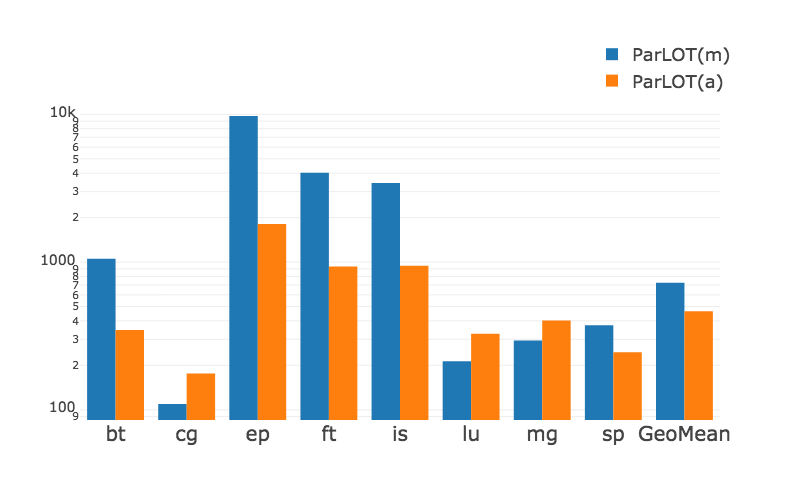
\includegraphics[width=3.8in]{figs.comet.newMed/comet_chartAvg_cr_B_p3_5.png}
\caption{ Average compression ratio of \parlot on the NPB applications - Input B}
\label{comet_chartAvg_cr_B_p3_5}
\end{figure}

\begin{figure}[t]
\centering
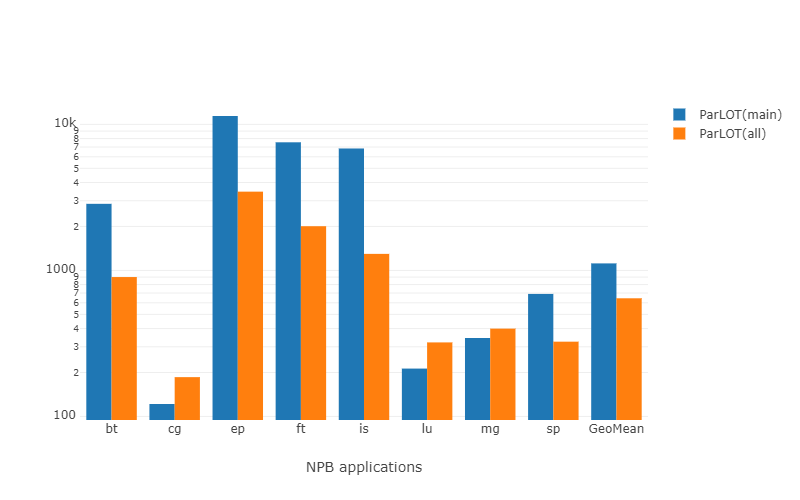
\includegraphics[width=3.8in]{figs.comet.newMed/comet_chartAvg_cr_C_p3_5.png}
\caption{ Average compression ratio of \parlot on the NPB applications - Input C}
\label{comet_chartAvg_cr_C_p3_5}
\end{figure}
%%%%%%%%%%%%%%%%%%%%%%%%%%%%%%%%%
% ENDDDD
%%%%%%%%%%%%%%%%%%%%%%%%%%%%%%%%%



\iffalse
\begin{table*}[]
\caption{Compression Ratio}
\label{comet_cr_pMpA_BC_itn_p3.5}\begin{center}
\begin{tabular}{lrrrrrrrrr}
\hline
              &      bt &     cg &       ep &       ft &       is &     lu &     mg &      sp &      GM \\
\hline
 pinMain.B.1  & 3035.93 &  94.35 & 12456.18 & 12173.49 &  9718.38 & 167.72 &  99.08 &  878.27 & 1255.17 \\
 pinMain.B.4  &  586.64 &  82.48 & 10368.41 &  1737.09 &   909.20 & 140.29 & 254.95 &  338.16 &  559.36 \\
 pinMain.B.16 &  346.66 & 113.28 &  8563.85 &  1077.35 &  1200.57 & 178.98 & 387.63 &  123.02 &  496.83 \\
 pinMain.B.64 &  252.24 & 147.78 &  7611.04 &  1122.62 &  1907.95 & 366.80 & 437.31 &  152.91 &  591.11 \\
 AVG          & 1055.37 & 109.47 &  9749.87 &  4027.64 &  3434.03 & 213.45 & 294.74 &  373.09 &  725.62 \\
 pinAll.B.1   &  514.51 & 137.41 &  3335.77 &  1226.74 &   543.18 & 314.63 & 260.87 &  303.88 &  500.21 \\
 pinAll.B.4   &  315.71 & 137.21 &  1266.92 &   436.15 &   316.16 & 287.25 & 329.57 &  199.66 &  330.70 \\
 pinAll.B.16  &  226.86 & 181.58 &  1246.66 &  1026.53 &   927.09 & 299.30 & 469.29 &  171.52 &  430.39 \\
 pinAll.B.64  &  329.23 & 247.30 &  1394.07 &  1043.94 &  1984.62 & 410.32 & 548.47 &  307.16 &  597.55 \\
 AVG          &  346.58 & 175.88 &  1810.86 &   933.34 &   942.76 & 327.88 & 402.05 &  245.56 &  464.71 \\
 pinMain.C.1  & 8618.95 & 111.16 & 13067.96 & 21335.57 & 21856.49 & 350.03 & 247.44 & 1977.43 & 2371.35 \\
 pinMain.C.4  & 1910.64 & 110.45 & 12418.66 &  6520.34 &  2256.56 & 112.77 & 267.98 &  472.68 &  928.16 \\
 pinMain.C.16 &  580.79 & 133.24 & 11017.36 &  1239.31 &  1347.88 & 164.47 & 396.86 &  143.13 &  582.78 \\
 pinMain.C.64 &  322.83 & 131.92 &  9154.99 &  1065.12 &  1896.25 & 223.69 & 465.74 &  168.89 &  585.74 \\
 AVG          & 2858.30 & 121.69 & 11414.74 &  7540.09 &  6839.30 & 212.74 & 344.50 &  690.53 & 1117.01 \\
 pinAll.C.1   & 2579.37 & 181.76 &  7376.96 &  5143.08 &  1520.42 & 408.21 & 314.77 &  650.73 & 1107.37 \\
 pinAll.C.4   &  448.61 & 161.32 &  3194.58 &  1062.94 &   527.34 & 274.70 & 319.35 &  237.43 &  477.42 \\
 pinAll.C.16  &  285.05 & 185.74 &  1765.49 &   588.86 &  1106.34 & 273.63 & 467.35 &  141.69 &  426.92 \\
 pinAll.C.64  &  290.00 & 214.68 &  1512.89 &  1237.30 &  2038.72 & 329.04 & 496.21 &  270.83 &  565.82 \\
 AVG          &  900.76 & 185.88 &  3462.48 &  2008.05 &  1298.21 & 321.39 & 399.42 &  325.17 &  644.38 \\
\hline
\end{tabular}
\end{center}
\end{table*}

\fi


\iftrue

\begin{table*}[]
\caption{ Compression ratio }
\label{comet_cr_pMpA_BC_itn_p3.5}\begin{center}
\npdecimalsign{.}
\nprounddigits{1}
\begin{tabular}{|c|c|c|N{5}{1}N{5}{1}N{5}{1}N{5}{1}N{5}{1}N{5}{1}n{5}{1}n{5}{1}|n{5}{1}|}
\hline
Input & Tool & \# Nodes  & \multicolumn{1}{c}{bt} & \multicolumn{1}{c}{cg} & \multicolumn{1}{c}{ep} & \multicolumn{1}{c}{ft} & \multicolumn{1}{c}{is} & \multicolumn{1}{c}{lu} & \multicolumn{1}{c}{mg} & \multicolumn{1}{c|}{sp} & \multicolumn{1}{c|}{GM} \\ \hline
\multirow{10}{*}{B} & \multirow{5}{*}{ParLOT(m)} & 1 & 3035.93 &  94.35 & 12456.18 & 12173.49 &  9718.38 & 167.72 &  99.08 &  878.27 & 1255.17 \\
 & & 4                                               &  586.64 &  82.48 & 10368.41 &  1737.09 &   909.20 & 140.29 & 254.95 &  338.16 &  559.36 \\
 & & 16                                              &  346.66 & 113.28 &  8563.85 &  1077.35 &  1200.57 & 178.98 & 387.63 &  123.02 &  496.83 \\
 & & 64                                              &  252.24 & 147.78 &  7611.04 &  1122.62 &  1907.95 & 366.80 & 437.31 &  152.91 &  591.11 \\ \cline{3-12} 
 & & AVG                                             & 1055.37 & 109.47 &  9749.87 &  4027.64 &  3434.03 & 213.45 & 294.74 &  373.09 &  {\boldmath}725.62  \\ \cline{2-12} 
 & \multirow{5}{*}{ParLOT(a)} & 1 &  514.51 & 137.41 &  3335.77 &  1226.74 &   543.18 & 314.63 & 260.87 &  303.88 &  500.21 \\
 & & 4                            &  315.71 & 137.21 &  1266.92 &   436.15 &   316.16 & 287.25 & 329.57 &  199.66 &  330.70 \\
 & & 16                           &  226.86 & 181.58 &  1246.66 &  1026.53 &   927.09 & 299.30 & 469.29 &  171.52 &  430.39 \\
 & & 64                           &  329.23 & 247.30 &  1394.07 &  1043.94 &  1984.62 & 410.32 & 548.47 &  307.16 &  597.55 \\ \cline{3-12} 
 & & AVG                          &  346.58 & 175.88 &  1810.86 &   933.34 &   942.76 & 327.88 & 402.05 &  245.56 &  {\boldmath}464.71 \\ \hline 
 \multirow{10}{*}{C} & \multirow{5}{*}{ParLOT(m)} & 1  & 8618.95 & 111.16 & 13067.96 & 21335.57 & 21856.49 & 350.03 & 247.44 & 1977.43 & 2371.35  \\
 & & 4                                                 & 1910.64 & 110.45 & 12418.66 &  6520.34 &  2256.56 & 112.77 & 267.98 &  472.68 &  928.16  \\
 & & 16                                                &  580.79 & 133.24 & 11017.36 &  1239.31 &  1347.88 & 164.47 & 396.86 &  143.13 &  582.78  \\
 & & 64                                                &  322.83 & 131.92 &  9154.99 &  1065.12 &  1896.25 & 223.69 & 465.74 &  168.89 &  585.74  \\ \cline{3-12} 
 & & AVG                                               & 2858.30 & 121.69 & 11414.74 &  7540.09 &  6839.30 & 212.74 & 344.50 &  690.53 & {\boldmath}1117.01  \\ \cline{2-12} 
 & \multirow{5}{*}{ParLOT(a)} & 1 & 2579.37 & 181.76 &  7376.96 &  5143.08 &  1520.42 & 408.21 & 314.77 &  650.73 & 1107.37 \\
 & & 4                            &  448.61 & 161.32 &  3194.58 &  1062.94 &   527.34 & 274.70 & 319.35 &  237.43 &  477.42 \\
 & & 16                           &  285.05 & 185.74 &  1765.49 &   588.86 &  1106.34 & 273.63 & 467.35 &  141.69 &  426.92 \\
 & & 64                           &  290.00 & 214.68 &  1512.89 &  1237.30 &  2038.72 & 329.04 & 496.21 &  270.83 &  565.82 \\ \cline{3-12}
 & & AVG                          &  900.76 & 185.88 &  3462.48 &  2008.05 &  1298.21 & 321.39 & 399.42 &  325.17 &  {\boldmath}644.38 \\ \cline{2-12} \hline
\end{tabular}
\npnoround
\end{center}
\end{table*}

\fi





\begin{figure}[t]
\centering
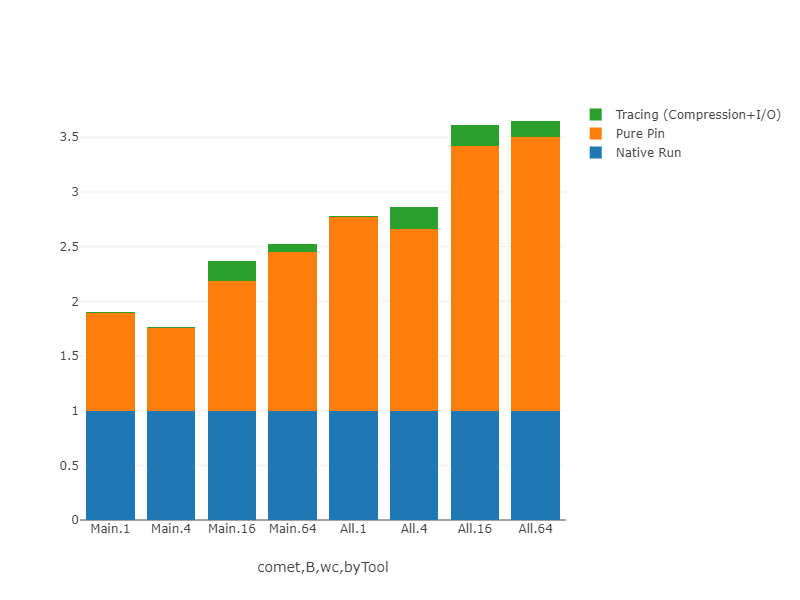
\includegraphics[width=3.8in]{figs.comet.newMed/comet_chartDet_B_wc_byTool_p3_5.png}
\caption{ Tracing overhead breakdown - Input B}
\label{comet_chartDet_B_wc_byTool_p3_5}
\end{figure}


\begin{figure}[t]
\centering
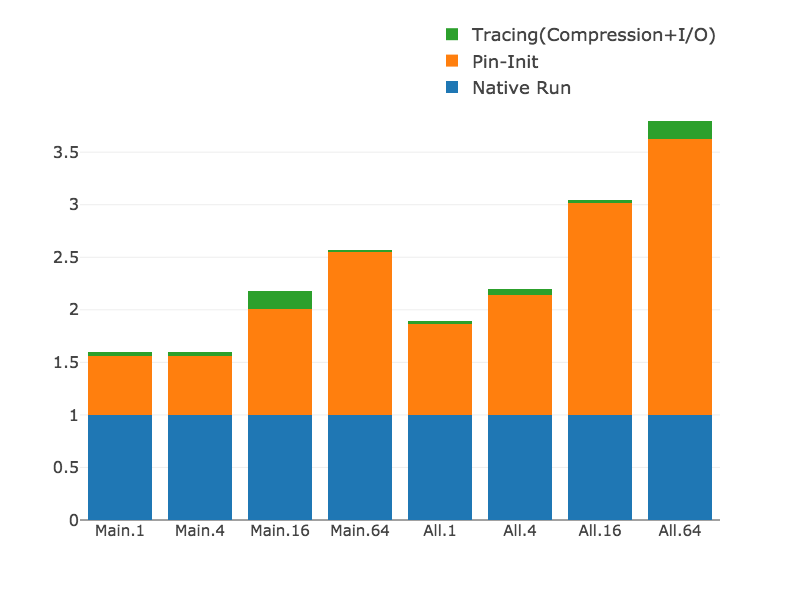
\includegraphics[width=3.8in]{figs.comet.newMed/comet_chartDet_C_wc_byTool_p3_5.png}
\caption{ Tracing overhead breakdown - Input C}
\label{comet_chartDet_C_wc_byTool_p3_5}
\end{figure}



\begin{figure}[t]
\centering
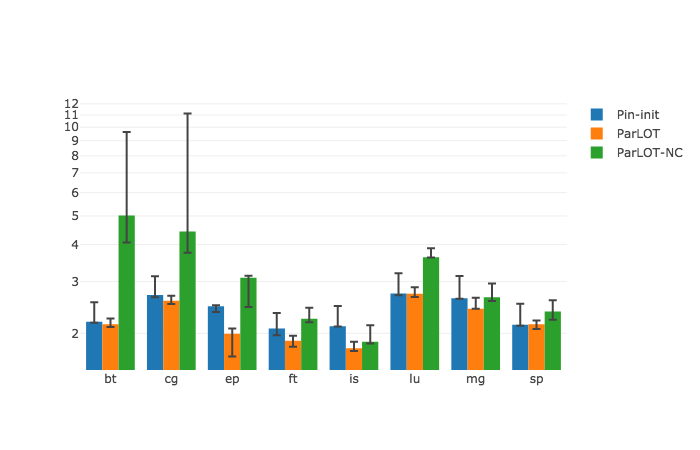
\includegraphics[width=3.7in]{figs.comet.newMed/comet_BX2_Main_16_B_p3_5.png}
\caption{ Variability of \parlotm overhead on 16 nodes - Input B}
\label{comet_BX2_Main_16_B_p3_5}
\end{figure}


%%%%%%%%%%%%%%%%%%%%%%%%%%%%%%%%%%%%%%%%%%%%%%%%%%%%%%%%%%%%%%%%%%%%%%%%%%%%%%%%%%
  
\subsection{Compression Ratio}
\label{subsec:cr}
Table \ref{comet_cr_pMpA_BC_itn_p3.5} shows the compression ratios for all configurations and inputs.
%
On average, \parlot stores between half a kilobyte and a kilobyte of trace info in a single byte. 
%
We observe that the
average compression ratio for \parlota input C is 644.3, and its
corresponding required bandwidth from Table
\ref{comet_bw_pMpAcg_BC_itn_p3.5} is 56.3.
%
This means \parlot can
collect \textbf{more than 36 MB} worth of data per core per second
while only needing 56 kB/s of the system bandwidth, {\em leaving the rest of the available bandwidth for application.}
%
In comparison, \callgrind only
collects \textbf{less than 100 kB} of data but still adds more
overhead compared to either \parlota or \parlotm . 
%
The average amount of trace data that can be collected by \parlota is
\textbf{360x} (85x for \parlotm) larger than that for \callgrind.
%
In the best observed case, the compression ratio of
\parlot exceeds 21000.
%
This is particularly impressive because it was achieved with relatively low overhead and incremental  
on-the-fly compression.
%
Generally, the compression ratios of \parlotm are higher than those of \parlota because the variety of distinct function calls on the main image is smaller than when tracing all images, thus compression performs better on \parlotm. 
Also by looking at Fig. \ref{comet_chartAvg_bw_B_p3_5}, Fig. \ref{comet_chartAvg_bw_C_p3_5}, Fig. \ref{comet_chartAvg_cr_B_p3_5} and Fig. \ref{comet_chartAvg_cr_C_p3_5}, we find EP to have the maximum compression ratio among the NPB applications. At the same time, it has the minimum required bandwidth. The opposite is true for CG, which exhibits the minimum compression ratio and the maximum required bandwidth. CG is a conjugate gradient method with irregular memory accesses and communications whereas EP is an embarrassingly parallel random number generator. CG's whole-program trace contains a larger number of distinct calls and more complex patterns than that of EP, thus resulting in a higher bandwidth and smaller compression ratio.
%

\parlot's ompression mechanism works better on larger input sizes because larger inputs tend to result in longer streams of similar function calls (e.g., a call that is made for every processed element)
  


  
%%%%%%%%%%%%%%%%%%%%%%%%%%%%%%%%%%%%%%%%%%%%%%%%%%%%%%%%%%%%%  

\begin{figure}[t]
\centering
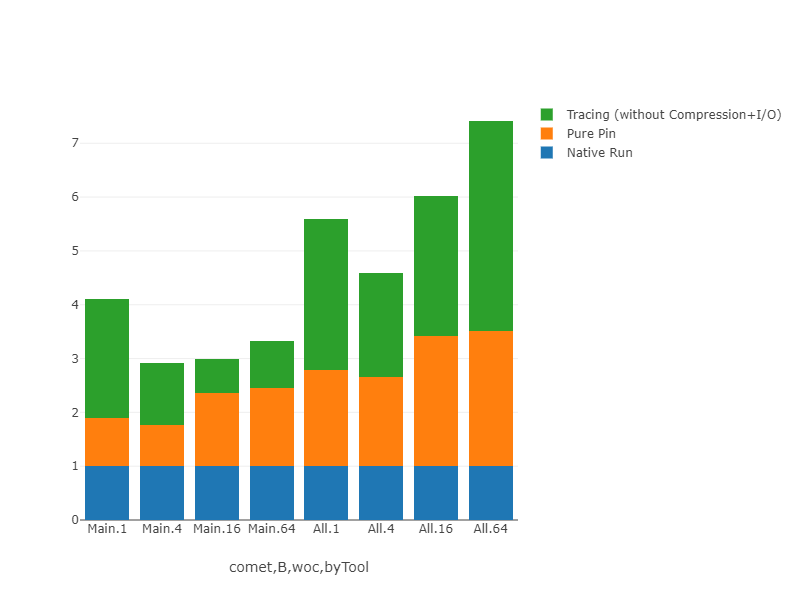
\includegraphics[width=3.8in]{figs.comet.newMed/comet_chartDet_B_woc_byTool_p3_5.png}
\caption{\parlotnc tracing overhead breakdown - Input B}
\label{comet_chartDet_B_woc_byTool_p3_5}
\end{figure}

\begin{figure}[t]
\centering
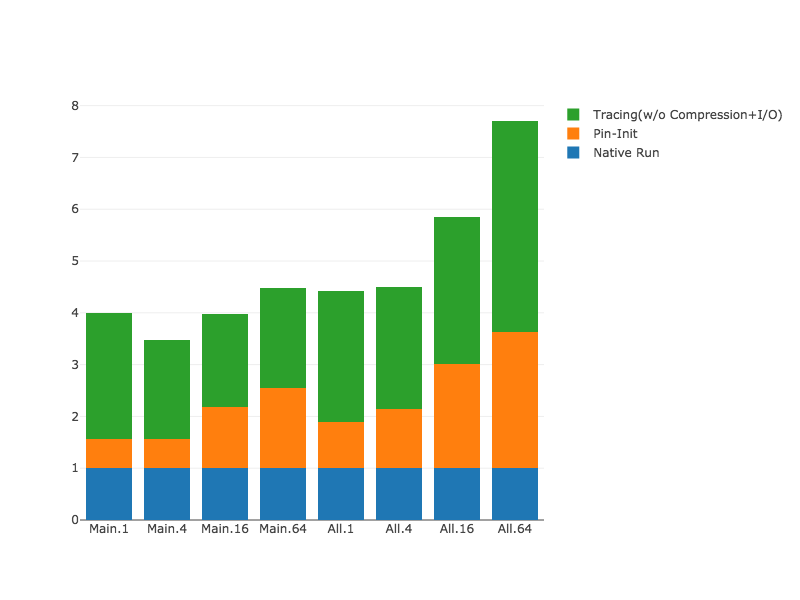
\includegraphics[width=3.8in]{figs.comet.newMed/comet_chartDet_C_woc_byTool_p3_5.png}
\caption{ \parlotnc tracing overhead breakdown - Input C}
\label{comet_chartDet_C_woc_byTool_p3_5}
\end{figure}

  
\subsection{Overheads} 
\label{subsec:pinit}
Tables \ref{comet_wo_det_Main_all_B_p3.5} and
\ref{comet_wo_det_All_all_B_p3.5} present the average overhead added on each
application for different versions of \parlot. 
%
The last row of these two tables
presents the geometric mean.
%
This information captures how much each
phase of \parlot slows down the native execution. 

\begin{table*}[]
\caption{Tracing overhead added by each version of \parlot - Input: B}
\begin{center}
\label{comet_wo_det_Main_all_B_p3.5}
\scalebox{0.80}{
\begin{tabular}{|c|c|rrr|rrr|rrr|rrr|} 
\hline 
\multicolumn{1}{|l|}{\multirow{2}{*}{\textbf{Input: B}}} & \multicolumn{1}{r|}{Nodes :}    & \multicolumn{3}{c|}{1}  & \multicolumn{3}{c|}{4} & \multicolumn{3}{c|}{16}  & \multicolumn{3}{c|}{64} \\ \cline{2-14} 
\multicolumn{1}{|l|}{} & \multicolumn{1}{r|}{Detail Tools:} & \multicolumn{1}{c}{\pininit} & \multicolumn{1}{c}{\parlot} & \multicolumn{1}{c|}{\parlotnc} & \multicolumn{1}{c}{\pininit} & \multicolumn{1}{c}{\parlot} & \multicolumn{1}{c|}{\parlotnc} & \multicolumn{1}{c}{\pininit} & \multicolumn{1}{c}{\parlot} & \multicolumn{1}{c|}{\parlotnc} & \multicolumn{1}{c}{\pininit} & \multicolumn{1}{c}{\parlot} & \multicolumn{1}{c|}{\parlotnc} \\
\hline
\multirow{9}{*}{Main} &  bt  &  1.50  &  1.55  &   5.62  &  1.74  &  1.76  &  5.06  &  2.19  & \cellcolor{blue!25} 2.15  &  5.02  &  1.83  &  2.10  &  3.52 \\
 &  cg  &  1.75  &  1.82  &   2.38  &  1.84  &  1.85  &  2.64  &  2.70  & \cellcolor{blue!25} 2.58  &  4.43  &  2.32  & \cellcolor{blue!25} 2.17  &  4.64 \\
 &  ep  &  2.96  & \cellcolor{blue!25} 2.62  &  20.48  &  1.99  & \cellcolor{blue!25} 1.89  &  5.38  &  2.47  & \cellcolor{blue!25} 1.99  &  3.09  &  2.68  & \cellcolor{blue!25} 2.39  &  2.66 \\
 &  ft  &  1.87  &  2.11  &   6.17  &  1.75  & \cellcolor{blue!25} 1.74  &  2.79  &  2.08  & \cellcolor{blue!25} 1.89  &  2.24  &  2.18  & \cellcolor{blue!25} 1.96  &  2.14 \\
 &  is  &  2.47  &  2.47  &   4.82  &  1.79  & \cellcolor{blue!25} 1.78  &  2.07  &  2.11  & \cellcolor{blue!25} 1.78  &  1.87  &  4.51  & \cellcolor{blue!25} 4.31  &  5.71 \\
 &  lu  &  1.32  & \cellcolor{blue!25} 1.31  &   1.44  &  1.75  &  1.77  &  2.25  &  2.73  &  2.73  &  3.62  &  3.05  &  4.39  &  6.13 \\
 &  mg  &  2.56  & \cellcolor{blue!25} 2.53  &   2.79  &  1.56  & \cellcolor{blue!25} 1.52  &  1.59  &  2.63  & \cellcolor{blue!25} 2.43  &  2.65  &  1.95  &  1.97  &  1.85 \\
 &  sp  &  1.34  & \cellcolor{blue!25} 1.33  &   2.43  &  1.73  &  1.73  &  3.58  &  2.14  &  2.15  &  2.37  &  1.95  &  2.07  &  2.54 \\
\cline{2-14}
 &  GM  &  1.89  &  1.90  &   4.10  &  1.77  & \cellcolor{blue!25} 1.75  &  2.92  &  2.37  & \cellcolor{blue!25} 2.19  &  3.00  &  2.45  &  2.52  &  3.33 \\
\hline 
\end{tabular} }

\end{center}
\end{table*}


\begin{table*}[]
\caption{Tracing overhead added by each version of \parlot - Input: B}
\begin{center}
\label{comet_wo_det_All_all_B_p3.5}
\scalebox{0.8}{
\begin{tabular}{|c|c|rrr|rrr|rrr|rrr|} 
\hline 
\multicolumn{1}{|l|}{\multirow{2}{*}{\textbf{Input: B}}} & \multicolumn{1}{r|}{Nodes :}    & \multicolumn{3}{c|}{1}  & \multicolumn{3}{c|}{4} & \multicolumn{3}{c|}{16}  & \multicolumn{3}{c|}{64} \\ \cline{2-14} 
\multicolumn{1}{|l|}{} & \multicolumn{1}{r|}{Detail Tools:} & \multicolumn{1}{c}{\pininit} & \multicolumn{1}{c}{\parlot} & \multicolumn{1}{c|}{\parlotnc} & \multicolumn{1}{c}{\pininit} & \multicolumn{1}{c}{\parlot} & \multicolumn{1}{c|}{\parlotnc} & \multicolumn{1}{c}{\pininit} & \multicolumn{1}{c}{\parlot} & \multicolumn{1}{c|}{\parlotnc} & \multicolumn{1}{c}{\pininit} & \multicolumn{1}{c}{\parlot} & \multicolumn{1}{c|}{\parlotnc} \\
\hline
\multirow{9}{*}{All} &  bt  &  1.76  &  1.84  &   6.11  &  2.39  &  2.57  &  6.11  &  3.22  &  3.52  &   9.02  &  2.87  &  3.14  &   7.55 \\
 &  cg  &  2.69  &  2.73  &   3.80  &  2.86  &  3.06  &  4.48  &  4.07  &  4.20  &  11.38  &  3.33  & \cellcolor{blue!25} 3.26  &  10.39 \\
 &  ep  &  4.36  & \cellcolor{blue!25} 4.18  &  22.20  &  3.14  &  3.41  &  7.16  &  3.12  &  3.39  &   4.55  &  4.18  & \cellcolor{blue!25} 3.83  &   4.16 \\
 &  ft  &  2.80  & \cellcolor{blue!25} 2.78  &   6.85  &  2.65  &  2.77  &  3.82  &  2.82  &  2.94  &   3.66  &  3.15  & \cellcolor{blue!25} 3.02  &   3.57 \\
 &  is  &  4.40  & \cellcolor{blue!25} 4.22  &   7.04  &  2.85  &  2.96  &  3.42  &  2.91  & \cellcolor{blue!25} 2.83  &   3.24  &  5.38  &  5.44  &   8.81 \\
 &  lu  &  1.70  &  1.73  &   2.39  &  2.54  &  2.76  &  4.88  &  3.96  &  4.30  &  10.47  &  4.45  &  4.65  &  23.41 \\
 &  mg  &  4.83  & \cellcolor{blue!25} 4.75  &   5.37  &  2.51  &  2.79  &  3.07  &  4.32  &  4.46  &   5.22  &  2.73  &  3.17  &   3.26 \\
 &  sp  &  1.70  &  1.72  &   3.01  &  2.46  &  2.66  &  5.06  &  3.27  &  3.65  &   5.67  &  2.77  &  3.31  &  11.65 \\
\cline{2-14}
 &  GM  &  2.78  & \cellcolor{blue!25} 2.77  &   5.59  &  2.66  &  2.86  &  4.58  &  3.42  &  3.62  &   6.02  &  3.51  &  3.65  &   7.41 \\
\hline 
\end{tabular} }

\end{center}
\end{table*}



In general, one 
expects the following inequality to hold:
 the overhead of \pininit should be less than that of \parlot
, which should be less than that of \parlotnc. 
%
This is not always the case because of the non-deterministic runtimes of the applications.
%
In fact, the variability across three runs of each experiment
is shown in Fig. \ref{comet_BX2_Main_16_B_p3_5}
where we present the minimum, maximum and median overheads.
%
These
overheads are for input size B and 16 nodes. 
%
This variability explains the seeming inconsistencies in  Tables
\ref{comet_wo_det_Main_all_B_p3.5} and
\ref{comet_wo_det_All_all_B_p3.5}.


On average, \pininit adds
an overhead of 3.28  and \parlota adds an overhead of 3.42. 
%
This means that \textbf{almost 96\%
of \parlota's overhead is due to \pin}. 
%
The results of \parlotm and
other inputs follow the same pattern
(as Fig. \ref{comet_chartDet_B_wc_byTool_p3_5} and \ref{comet_chartDet_C_wc_byTool_p3_5} show). 
%
The overhead that \parlot (excluding the overhead of \pininit) {\em adds}
to the applications is very small.
%
If we were to switch to a different
instrumentation tool that is not as general as \pin but more
lightweight, the overhead would potentially reduce drastically. \\


\subsection{Compression Impact} 
\label{subsec:compact}

Fig. \ref{comet_chartDet_B_woc_byTool_p3_5} and Fig. \ref{comet_chartDet_C_woc_byTool_p3_5} show the breakdown overhead by \parlotnc which illustrate the impact of compression; they also highlight the importance of incorporating compression directly in the tracing tool. 
%
On average, \parlotnc slows down the application execution almost \textbf{2x} more than \parlota. 
%
The average overhead 
across Table \ref{comet_wo_det_All_all_B_p3.5} for \parlota is \textbf{3.4}.
%
The  corresponding factor for \parlotnc is \textbf{6.6}. 
%
The numbers of \parlotm and input C  follow the same pattern. For example, \parlotnc slows down the application execution almost \textbf{1.66x} more than \parlotm.
%

Clearly, compression not only lowers the storage requirement but also the overhead. This is important as it shows that the extra computation to perform the compression is more than amortized by the reduction in the amount of data that need to be written out.
%

This result validates our approach and highlights that incremental, on-the-fly compression is likely essential to make whole-program tracing possible at low overhead.